\section{Synchronizing the time}

Because the clients may run on different computers the computer clock time cannot be used as a parameter to the animations since the computer clocks are unlikely to be in sync with each other. As shown in chapter 1 this is a well known problem in distributed systems, so the first step would be to implement one or several existing algorithms. 

A combination of the Berkley algoritm (ref section) and NTP (ref section) was used to synchronize the time of the clients and the server. Both NTP and the Berkley algorithm are designed to be used in intranets since they assume an evenly distributed delay. The end product that the work in this thesis will be used for was assumed to run on an intranet. The accuracy given by these algoritms was assumed to be good enough. 

An artificial time is created both on the server and the clients on start but this time never changed, instead a delta value added with to the artificial time is used for input to the animations.  

\subsection {Distributing deltas}

The server initiates the synchronization with the clients by sending a sync event as a message to the clients. The clients replies with the time they recieved the message, the time they send their reply and the clients old delta-value. The server then calculates each clients delta and sends each client a message containing their new delta. 

If the value of the old delta of the client and the new delta calculated by the server differs more than 2 milliseconds the server will send a new sync event as a message to the client, repeating the procedure until the delta is stable. 

Everytime a new client connects to the server this client needs to synchronize its time with the server. 

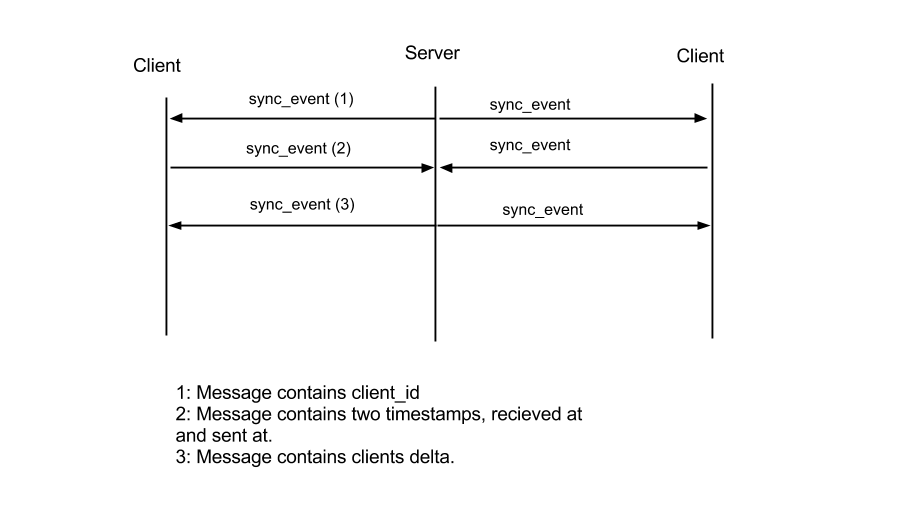
\includegraphics[width=1.0\textwidth]{figures/comm.png}

\subsection{Calculating deltas}
An implementation of NTP was used to calculate each clients latency, shown below.

\begin{verbatim}
self.delta = ((self.t_1 - self.t_0) + (self.t_2 - self.t_3))/2
\end{verbatim}

\subsection {Using the delta values}

All animations must take a timestamp as a parameter for playback. This will be used to timestep through the animation. To create this timestamp the client uses the time it gets when it adds its delta value to its own local time. This way all clients will be at the same place in the animation, at the same time, given that they have a correct delta value. 


